\usetikzlibrary{shapes.arrows}
\definecolor{redtop}{HTML}{ffebee}
\definecolor{redfront}{HTML}{ffebee}
\definecolor{redright}{HTML}{ffcdd2}
\definecolor{redline}{HTML}{ef9a9a}

\definecolor{bluetop}{HTML}{e0f7fa}
\definecolor{bluefront}{HTML}{e0f7fa}
\definecolor{blueright}{HTML}{b2ebf2}
\definecolor{blueline}{HTML}{80deea}

\definecolor{greentop}{HTML}{e8f5e9}
\definecolor{greenfront}{HTML}{e8f5e9}
\definecolor{greenright}{HTML}{c8e6c9}
\definecolor{greenline}{HTML}{a5d6a7}

\definecolor{yellowtop}{HTML}{fff176}
\definecolor{yellowfront}{HTML}{fff176}
\definecolor{yellowright}{HTML}{ffee58}
\definecolor{yellowline}{HTML}{ffeb3b}

\definecolor{orangetop}{HTML}{fffde7}
\definecolor{orangefront}{HTML}{fff3e0}
\definecolor{orangeright}{HTML}{ffe0b2}
\definecolor{orangeline}{HTML}{ffcc80}

\definecolor{browntop}{HTML}{efebe9}
\definecolor{brownfront}{HTML}{efebe9}
\definecolor{brownright}{HTML}{d7ccc8}
\definecolor{brownline}{HTML}{bcaaa4}

\definecolor{darkbluetop}{HTML}{f5f5f5}
\definecolor{darkbluefront}{HTML}{eeeeee}
\definecolor{darkblueright}{HTML}{e0e0e0}
\definecolor{darkblueline}{HTML}{bdbdbd}

\definecolor{purpletop}{HTML}{f3e5f5}
\definecolor{purplefront}{HTML}{f3e5f5}
\definecolor{purpleright}{HTML}{e1bee7}
\definecolor{purpleline}{HTML}{ce93d8}

\newcommand\cube[7]{
    \ifstrequal{#7}{blue}{
        \def\top{bluetop}
        \def\front{bluefront}
        \def\right{blueright}
        \def\line{blueline}
    }{\ifstrequal{#7}{red}{
        \def\top{redtop}
        \def\front{redfront}
        \def\right{redright}
        \def\line{redline}
    }{\ifstrequal{#7}{yellow}{
        \def\top{yellowtop}
        \def\front{yellowfront}
        \def\right{yellowright}
        \def\line{yellowline}
    }{\ifstrequal{#7}{orange}{
        \def\top{orangetop}
        \def\front{orangefront}
        \def\right{orangeright}
        \def\line{orangeline}
    }{\ifstrequal{#7}{green}{
        \def\top{greentop}
        \def\front{greenfront}
        \def\right{greenright}
        \def\line{greenline}
    }{\ifstrequal{#7}{brown}{
        \def\top{browntop}
        \def\front{brownfront}
        \def\right{brownright}
        \def\line{brownline}
    }{\ifstrequal{#7}{darkblue}{
        \def\top{darkbluetop}
        \def\front{darkbluefront}
        \def\right{darkblueright}
        \def\line{darkblueline}
    }{\ifstrequal{#7}{purple}{
        \def\top{purpletop}
        \def\front{purplefront}
        \def\right{purpleright}
        \def\line{purpleline}
    }{
        \def\top{bluetop}
        \def\front{bluefront}
        \def\right{blueright}
        \def\line{blueline}
    }}}}}}}}
    \fill[fill=\front,draw=\line,shift={(0,0,0)}](#1,#2,#3)--(#1+#4,#2,#3)--(#1+#4,#2+#5,#3)--(#1,#2+#5,#3)--cycle;
    \fill[fill=\top,draw=\line,shift={(0,#5,0)}](#1,#2,#3)--(#1+#4,#2,#3)--(#1+#4,#2,#3-#6)--(#1,#2,#3-#6)--cycle;
    \fill[fill=\right,draw=\line,shift={(#4,0,0)}](#1,#2,#3)--(#1,#2,#3-#6)--(#1,#2+#5,#3-#6)--(#1,#2+#5,#3)--cycle;
}

\newcommand\featuremap[1]{
    \cube{0}{0}{0}{8}{24}{6}{#1}
    \foreach \x in {0, ..., 7} {
        \foreach \y in {0, ..., 23} {
            \cube{\x}{\y}{0}{1}{1}{1}{#1}
        }
    }
}

\newcommand\pcb{
    \foreach \x in {0, ..., 7} {
        \foreach \y in {0, ..., 3} {
            \cube{\x}{\y+0}{0}{1}{1}{6}{blue}
            \cube{\x}{\y+0}{0}{1}{1}{1}{blue}
        }
    }
    \foreach \x in {0, ..., 7} {
        \foreach \y in {0, ..., 3} {
            \cube{\x}{\y+4}{0}{1}{1}{6}{red}
            \cube{\x}{\y+4}{0}{1}{1}{1}{red}
        }
    }
    \foreach \x in {0, ..., 7} {
        \foreach \y in {0, ..., 3} {
            \cube{\x}{\y+8}{0}{1}{1}{6}{purple}
            \cube{\x}{\y+8}{0}{1}{1}{1}{purple}
        }
    }
    \foreach \x in {0, ..., 7} {
        \foreach \y in {0, ..., 3} {
            \cube{\x}{\y+12}{0}{1}{1}{6}{green}
            \cube{\x}{\y+12}{0}{1}{1}{1}{green}
        }
    }
    \foreach \x in {0, ..., 7} {
        \foreach \y in {0, ..., 3} {
            \cube{\x}{\y+16}{0}{1}{1}{6}{brown}
            \cube{\x}{\y+16}{0}{1}{1}{1}{brown}
        }
    }
    \foreach \x in {0, ..., 7} {
        \foreach \y in {0, ..., 3} {
            \cube{\x}{\y+20}{0}{1}{1}{6}{orange}
            \cube{\x}{\y+20}{0}{1}{1}{1}{orange}
        }
    }
    \foreach \y in {0, ..., 5} {
        \draw[draw=black, line width=0.06em, shift={(0, 4*\y, 0)}] (0,0) -- (8,0) -- (8,4) -- (0,4) -- cycle;
    }
}

\newcommand\colvector{
    \cube{0}{1.5+0 }{0}{1}{1}{6}{blue}
    \cube{0}{1.5+4 }{0}{1}{1}{6}{red}
    \cube{0}{1.5+8 }{0}{1}{1}{6}{purple}
    \cube{0}{1.5+12}{0}{1}{1}{6}{green}
    \cube{0}{1.5+16}{0}{1}{1}{6}{brown}
    \cube{0}{1.5+20}{0}{1}{1}{6}{orange}
    \foreach \y in {0, ..., 5} {
        \draw[draw=black, line width=0.06em, shift={(0, 1.5+4*\y, 0)}] (0,0) -- (1,0) -- (1,1) -- (0,1) -- cycle;
    }
}

\newcommand\classify[3]{
    \draw[draw=#3,line width=0.15em,rounded corners=0.4em] (#1-3,#2-3) rectangle (#1+21,#2+3);
    \draw[line width=0.15em] (#1+0,#2+0) circle[radius=2];
    \draw[line width=0.15em] (#1+6,#2+0) circle[radius=2];
    \draw[font=\fontsize{20em}{6}\selectfont] node at (#1+12,#2+0) {...};
    \draw[line width=0.15em] (#1+18,#2+0) circle[radius=2];
}

\newcommand\softmax{
    \classify{0}{0}{blueline}
    \classify{0}{8}{redline}
    \classify{0}{16}{purpleline}
    \classify{0}{24}{greenline}
    \classify{0}{32}{brownline}
    \classify{0}{40}{orangeline}
}

\newcommand\notes[3]{
    \node[draw, single arrow,
          minimum height=11em, minimum width=8em,
          single arrow head extend=0.5em,
          anchor=west] at (#1,#2) {};
    \node[font=\fontsize{5em}{6}\selectfont] at (#1+1.5, #2+3) {#3};
}

\tikzset{global scale/.style={
    scale=#1,
    every node/.append style={scale=#1}
}}

\newcommand\figarchpcb{
    \begin{tikzpicture}[line join=round, line width=0.05em, global scale=0.18]
        \begin{scope}[shift={(0,1.5,0)}]
            \node[anchor=south west]{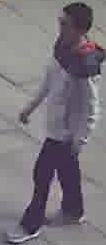
\includegraphics[width=26em]{person}};
        \end{scope}
        \begin{scope}[shift={(20,0,0)}]
            \featuremap{darkblue}
        \end{scope}
        \begin{scope}[shift={(40,0,0)}]
            \pcb
        \end{scope}
        \begin{scope}[shift={(60,0,0)}]
            \colvector
        \end{scope}
        \begin{scope}[shift={(75,3,0)},global scale=0.5]
            \softmax
        \end{scope}
        \notes{13}{12}{ResNet50}
        \notes{33}{12}{均匀分块}
        \notes{53}{12}{区域池化}
        \notes{66.5}{23}{}
        \notes{66.5}{19}{}
        \notes{66.5}{15}{}
        \notes{66.5}{11}{}
        \notes{66.5}{7}{}
        \notes{66.5}{3}{}
        \node[font=\fontsize{5em}{6}\selectfont] at (68, 26) {分类};
    \end{tikzpicture}
}